\documentclass{beamer}
\mode<presentation>
{
  \usetheme{Montpellier}
%  \setbeamercovered{transparent}
  \setbeamercovered{invisible}
}
\usepackage[english]{babel}
\usepackage[latin1]{inputenc}
\usepackage{graphicx,times,tkz-graph,mathrsfs,listings,verbatim,tikz,caption,amsmath,bm}
\usetikzlibrary{shapes.geometric}%   
\usepackage[T1]{fontenc}
\newcommand{\E}{\operatorname{E}}
\newcommand{\VE}{\operatorname{VE}}
\lstset{
	numberstyle=\footnotesize,
	basicstyle=\ttfamily\tiny}
\graphicspath{{WIgraphs/}}
%\graphicspath{{C:/Users/VOR1/Dropbox/Misc work/Waning immunity/WI project/WIgraphs/}}
%%%%%%%%%%%%%%%%%%%%%%%%%%%%%%%%%%%%%%%%%%%%%%%%%%%%%%%%%%%%%%%5
\title[Waning] % (optional, use only with long paper titles)
{``Intra-Seasonal Waning'' as Methodological Artifact}
\date{10/10/2018}
%
%
\author{Ivo M. Foppa}
% If you wish to uncover everything in a step-wise fashion, uncomment
% the following command:
%\beamerdefaultoverlayspecification{<+->}
\begin{document}
%
	\begin{frame}
	\titlepage
	\end{frame}
%
%
\section{Overview}
%
\section{Methdological sources of ``waning effect''}
\begin{frame}
Lipsitch editiorial (CID, 2018):
\begin{itemize}
	\item<2->[] ``Even if the vaccine effect does not wane over time, then such waning will nonetheless appear to occur in most studies [\ldots]'' (``leaky'' vaccines)
	\item<3->[] This will happen if:\begin{enumerate}
		\item<4-> ``there is heterogeneous risk of becoming infected within those who are vaccinated''
		\item<5-> ``some trial participants during the course of the trial become infected but are not counted as cases'' \uncover<6->{\textbf{$\leftarrow$ Not relevant to TND studies!}} 
		\item<7-> What if the vaccine is not leaky?
	\end{enumerate}
\end{itemize}
\end{frame}
\begin{frame}{Vaccine models}
\begin{itemize}
\item ``Leaky'' model: Those susceptible before vaccination have a risk of $\lambda_1 = \lambda_0 k$ of becoming infected during a contact if an unvaccinated susceptible has risk $\lambda_0$. $\operatorname{VE}=1-\frac{\lambda_1}{\lambda_0} = k$
\item<2-> ``All-or-none'' model: A proportion of those vaccinated becomes fully immunized against ``influenza virus'', while the rest remains fully susceptible
\item<3-> Hybrid models: \begin{enumerate}
	\item <4-> A \textbf{\emph{proportion}} of vaccinated develops ``leaky'' immunity (Lewnard, 2018)
	\item <5-> ``Leaky'' model with time-variant $k$ \uncover<7->{$\bm{\leftarrow}$}
	\item <6-> \ldots
\end{enumerate}
\end{itemize}
\end{frame}
%
%
\subsection{Approach}
\begin{frame}{Approach}
%
\begin{enumerate}
	\item 	\begin{itemize}
		\item<2-> Simulation of seasonal influenza epidemics using simple SIR ODE models
		\item<3-> Implement two scenarios (``leaky'', ''all-or-none'' with two viruses)
		\item<4-> Use numerical solutions to ODEs to generate TND data
		\item<5-> Calculate VE ``estimates'' and true VE
	\end{itemize}
	\item<6-> 	\begin{itemize}
	\item Simulation of seasonal influenza epidemics using a stochastic SIR model, keeping track of time since vaccination
	\item Implement ''all-or-none'' with two viruses: A certain proportion of the population 
	\item Use Ray's analytic approach (only vaccinees, conditional logistic regression)
\end{itemize}
\end{enumerate}
\end{frame}
%
\section{Results}
\subsection{``Leaky''}
\begin{frame}{First scenario: ``Leaky'' vaccine}
\centering
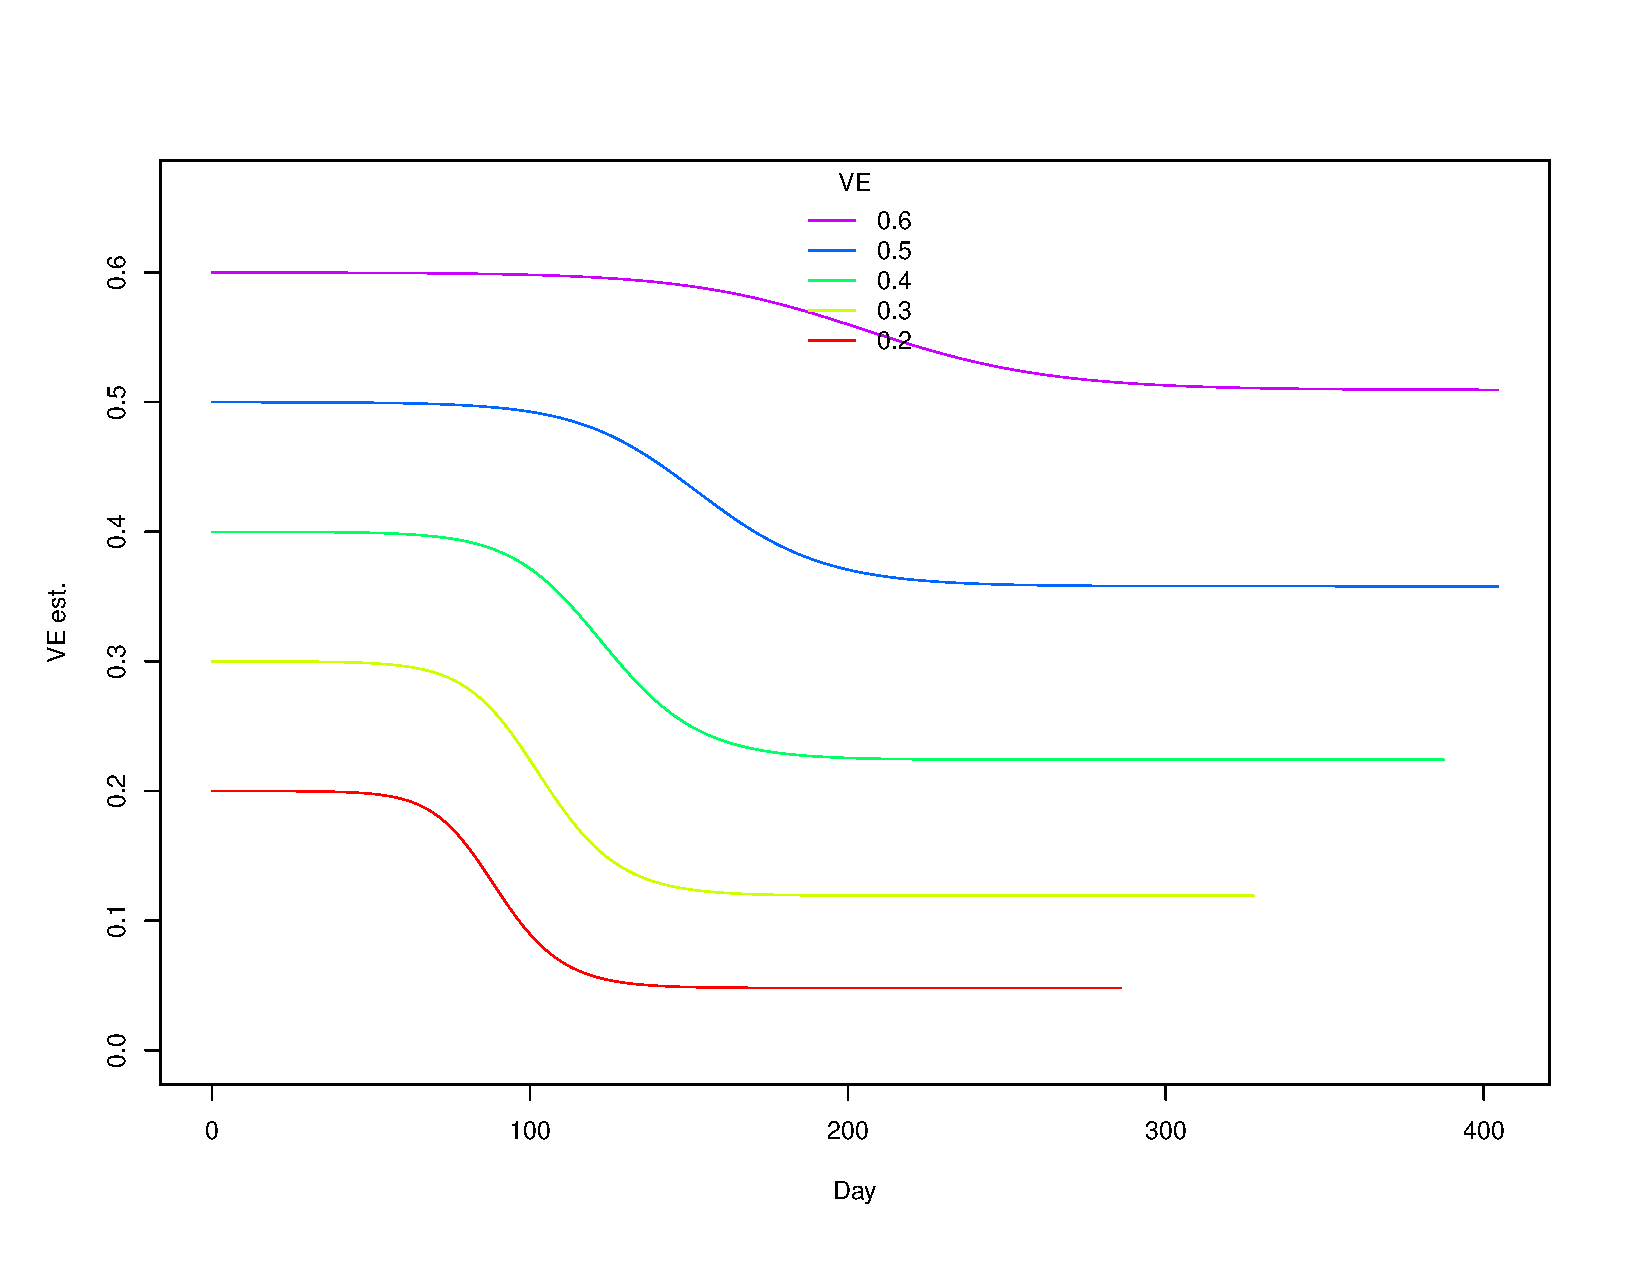
\includegraphics[width=.7\textwidth]{VEtime.pdf}
\end{frame}
%
%
\begin{frame}{Rel. Bias}
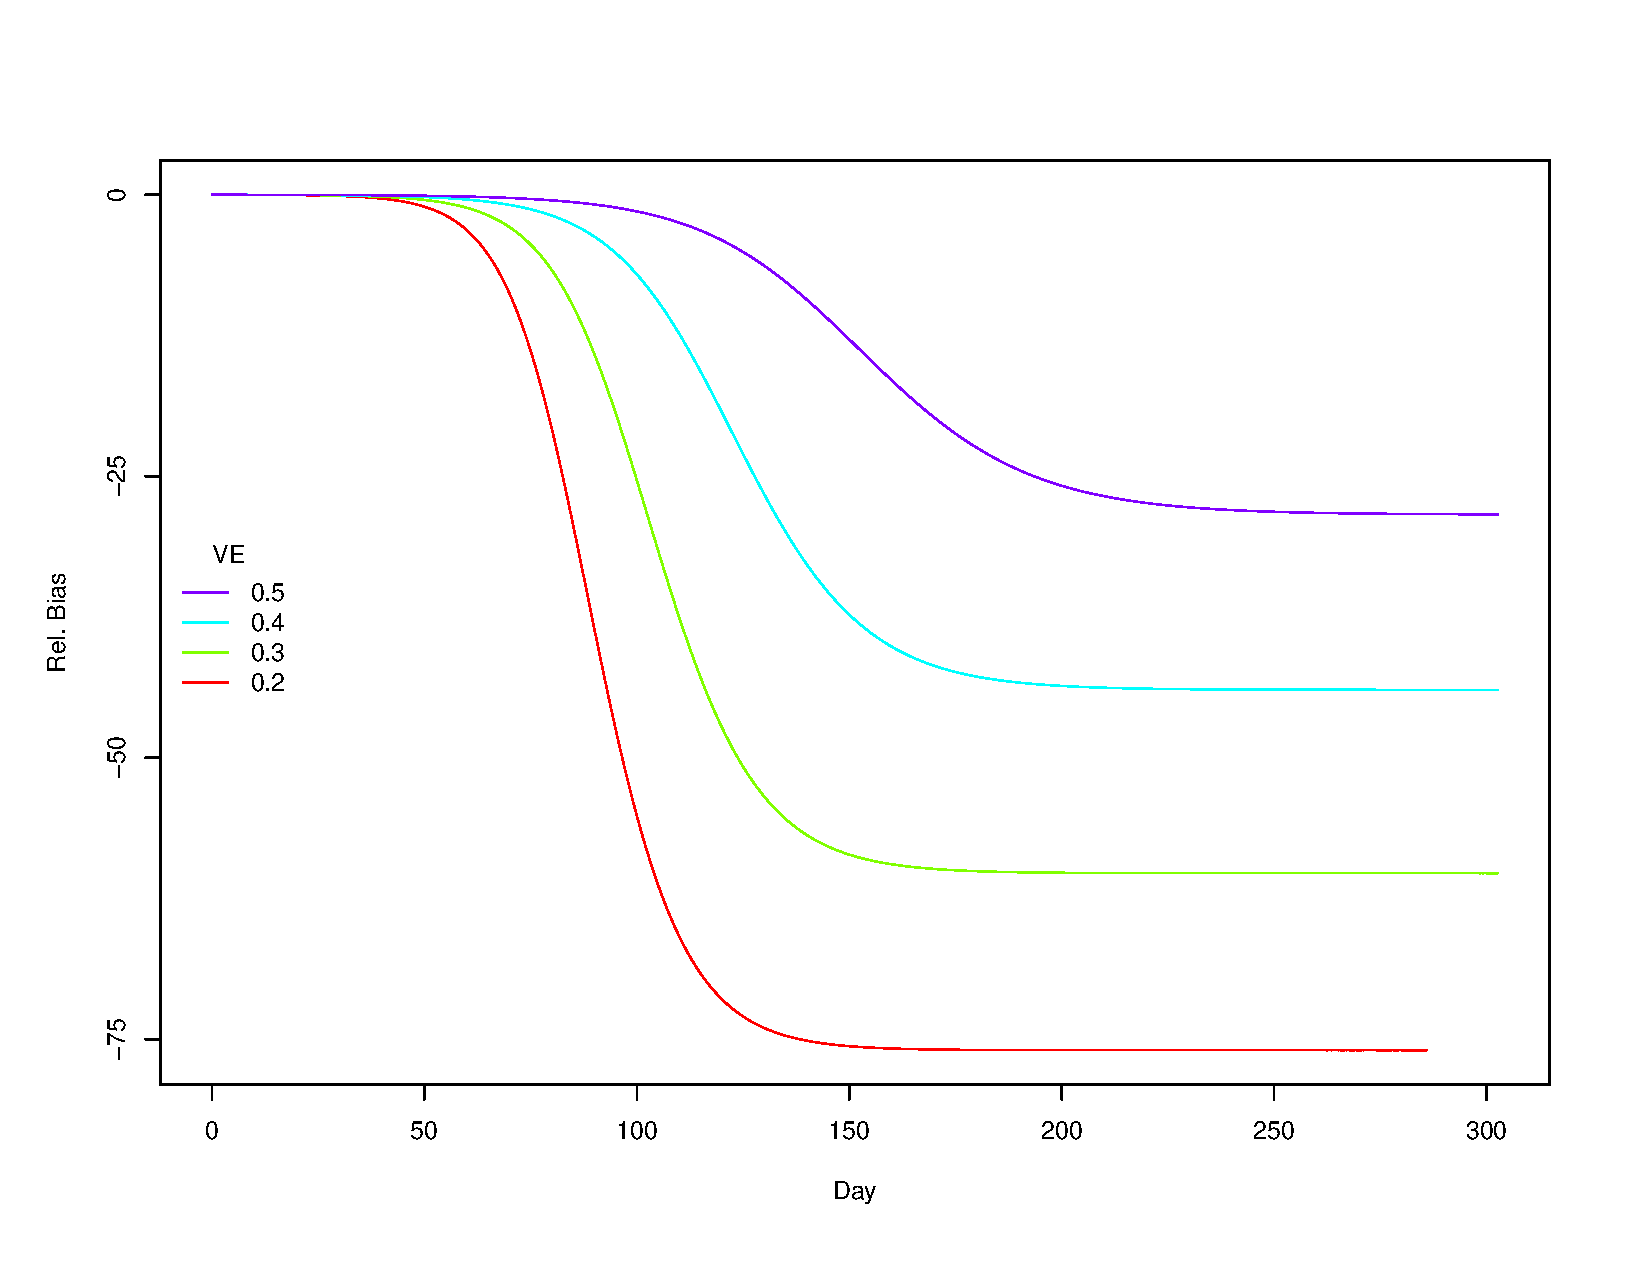
\includegraphics[width=.7\textwidth]{VEbias_rel.pdf}
\end{frame}
%
%
\subsection{``All-or-none'', 2 viruses}
\begin{frame}{Second scenario: 2 viruses, ``all-or-none''}
\centering
		\includegraphics[width=.7\textwidth]{VE_2_virus.pdf}
\end{frame}
%
\begin{frame}{Time-dependent ``k''}
\centering
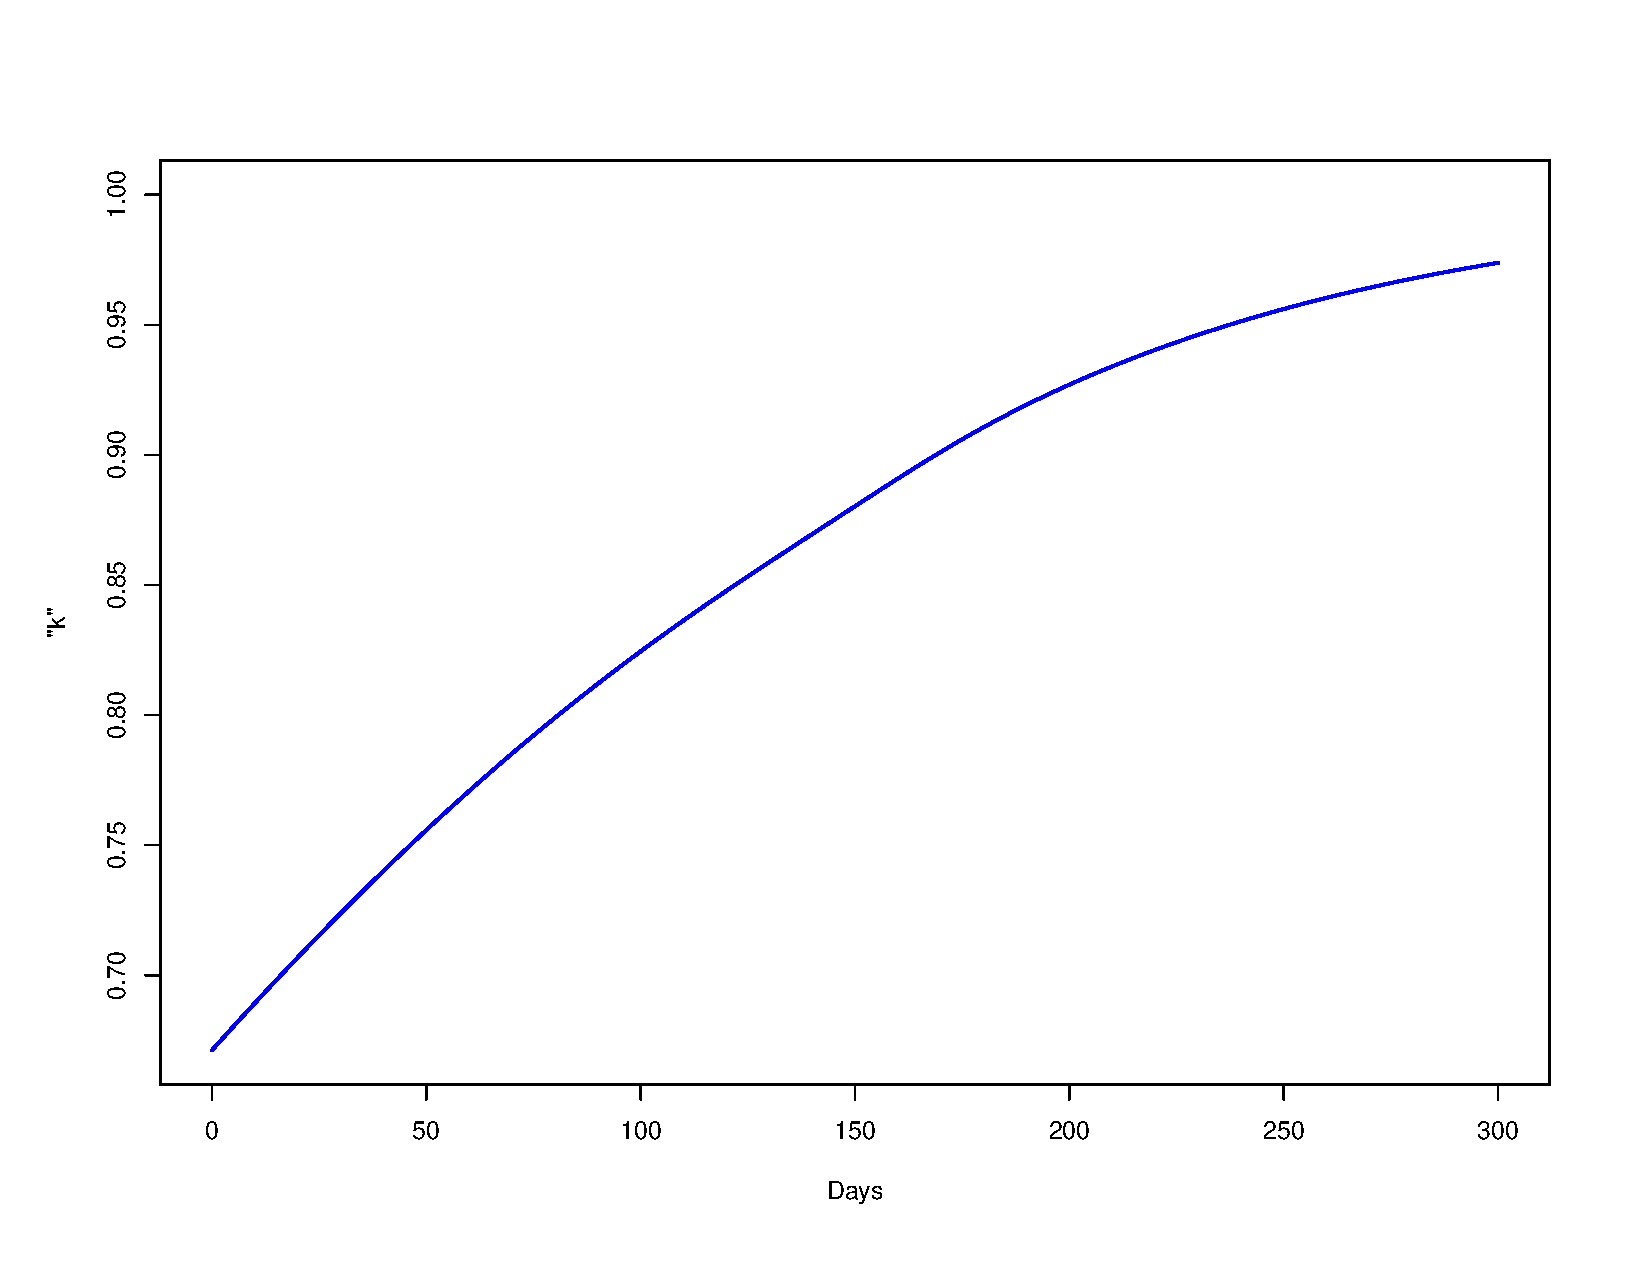
\includegraphics[width=.7\textwidth]{k_time.pdf}
\end{frame}
\end{document}
